\documentclass[12pt]{article}

\usepackage[english]{babel}
\usepackage[utf8x]{inputenc}
\usepackage[T1]{fontenc}
\usepackage{float}
\usepackage[sc,osf]{mathpazo}  
\linespread{1.025}
\usepackage{fancyvrb}
\usepackage[a4paper,top=2cm,bottom=2.25cm,left=2cm,right=2cm,marginparwidth=2cm]{geometry}
\usepackage{amsmath}
\usepackage{graphicx}
\usepackage[colorinlistoftodos]{todonotes}
\usepackage{enumitem}
\usepackage{listings}
\usepackage{authblk}
\usepackage{fancyhdr}
\usepackage{parskip}
\usepackage{fancyhdr}
\usepackage{vmargin}
\usepackage{tabu}
\author{Sakib Hasan}
\setpapersize{A4}
\setmarginsrb{25mm}{25mm}{25mm}{25mm}{0pt}{0mm}{0pt}{0mm}
\definecolor{dkgreen}{rgb}{0,0.6,0}
\definecolor{gray}{rgb}{0.5,0.5,0.5}
\definecolor{mauve}{rgb}{0.58,0,0.82}

\lstset{frame=tb,
  language= C++,
  aboveskip=3mm,
  belowskip=3mm,
  showstringspaces=false,
  columns=flexible,
  basicstyle={\small\ttfamily},
  numbers=none,
  numberstyle=\tiny\color{gray},
  keywordstyle=\color{blue},
  commentstyle=\color{dkgreen},
  stringstyle=\color{mauve},
  breaklines=true,
  breakatwhitespace=true,
  tabsize=3
}


%\title{Dynamic Programming- DP}	% Title

\begin{document}

\begin{titlepage}
\centering
\vspace{10mm}

\includegraphics[scale = 0.1]{logo.png}\\[1.5 cm]	% University Logo
%\textsc{\LARGE University of Dhaka\newline}\\[2.0 cm]	% University Name
\begin{center}\textbf{\LARGE University of Dhaka}\end{center}
\textsc{\Large Department of Computer Science and Engineering}\\[0.5 cm]
\begin{center} Design and Analysis of Algorithm \end{center}	% Course Code
	\rule{\linewidth}{0.2 mm} \\[0.4 cm]
	{ \huge \bfseries{Dynamic Programming- DP}}\\
	\rule{\linewidth}{0.2 mm} \\[1.5 cm]
	
	\begin{minipage}{0.4\textwidth}
		\begin{flushleft} \large
			\emph{Submitted To:}\\
			\vspace{6mm}
			Hasnain Heickal\\
           		 Asst. Professor\\
           		 Department of Computer Science and Engineering\\
			\end{flushleft}
			\end{minipage}~
			\begin{minipage}{0.4\textwidth}
            
			\begin{flushright} \large
			\emph{Submitted By :} \\
			\vspace{6mm}
			Sakib Hasan\\
           		 Roll : 149\\
			\vspace{6mm}
            		Tammana Sultana\\
            		Roll : 61\\
		\end{flushright}
       
	\end{minipage}\\[10mm]
	
\end{titlepage}
  \newpage
  %\pagenumbering{num_style}
  \section{What is Dynamic Programming?}
  Dynamic programming is an \textbf{optimization} approach that transforms a complex problem into a sequence of simpler problems; its essential characteristic is the multistage nature of the
  optimization procedure. More so than the optimization techniques described previously, dynamic programming provides a general framework for analyzing many problem types. Within this
  framework a variety of optimization techniques can be employed to solve particular aspects of a more general formulation. Usually creativity is required before we can recognize that a
  particular problem can be cast effectively as a dynamic program; and often subtle insights are necessary to restructure the formulation so that it can be solved effectively.\vspace{3mm} 
  \newline  \textbf{In easier words, Dynamic problem(DP) refers to simplifying a complicated problem by breaking it down into simpler sub-problems in a recursive manner.}

\subsection{General Concepts}
Let us learn about some general concepts before diving in to dynamic programming.

\begin{itemize}[label=$\diamond$]
\item Algorithm strategies
\begin{itemize}
\item Approach to solving a problem
\item May combine several approaches
\end{itemize}
\item Algorithm structures
\begin{itemize}
\item Iterative $\Rightarrow $ execute action in loop
\item Recursive  $\Rightarrow$ reapply action to sub-problem(s)
\end{itemize}
\item Problem types
\begin{itemize}
\item Decision $\Rightarrow$ find Yes/No answer
\item Satisfying $\Rightarrow$ find any satisfactory solution
\item Optimization $\Rightarrow$ find best solutions (vs. cost metric)
\end{itemize}
\end{itemize}
Now, dynamic programming is an algorithmic strategy where we try to break the original problem into smaller similar sub-problems and try to find optimal solution in recursive manner which refers to optimization. DP is based on remembering past results, so we also have to store already calculated data from smaller sub-problems solution. DP is generally used to solve \textbf{'Optimization Problems'}.

\subsection{Approach -}
\begin{enumerate}[label=(\roman*)]
\item Divide problem into smaller sub-problems 
\begin{itemize}
\item Sub-problems must be of same type
\item Sub-problems must overlap
\end{itemize}
\item Solve each sub-problem recursively
\begin{itemize}
\item May simply look up solution
\end{itemize}
\item Combine solutions into to solve original problem
\item Store solution to problem ( \textbf{'Tabulation'}  or \textbf{'Memoization'})
\end{enumerate}
\vspace{3mm} 

\subsection{Two key ingredients of dynamic programming}
\begin{enumerate}
\item Optimal substructures
\item Overlapping sub-problems
\end{enumerate}

\textbf{Optimal substructures} :
\par{\indent A given problems has Optimal Substructure Property if optimal solution of the given problem can be obtained by using optimal solutions of its subproblems.
\newline For example, the Shortest Path problem has following optimal substructure property:
\newline If a node x lies in the shortest path from a source node u to destination node v then the shortest path from u to v is combination of shortest path from u to x and shortest path from x to v. The standard All Pair Shortest Path algorithms like Floyd–Warshall and Bellman–Ford are typical examples of Dynamic Programming.}\vspace{2mm}

On the other hand, the Longest Path problem doesn’t have the Optimal Substructure property. Here by Longest Path we mean longest simple path (path without cycle) between two nodes. Consider the following unweighted graph. There are two longest paths from q to t: q→r→t and q→s→t. Unlike shortest paths, these longest paths do not have the optimal substructure property. For example, the longest path q→r→t is not a combination of longest path from q to r and longest path from r to t, because the longest path from q to r is q→s→t→r and the longest path from r to t is r→q→s→t.
\begin{figure}[H]
\centering
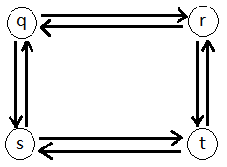
\includegraphics[width=0.25\textwidth]{longestpath.png}
\caption{\label{fig:graph_1}Sample Graph.}
\end{figure}
\vspace{6mm}
\textbf{Overlapping sub-problems} :
\par{\indent Like Divide and Conquer, Dynamic Programming combines solutions to sub-problems. Dynamic Programming is mainly used when solutions of same subproblems are needed again and again. In dynamic programming, computed solutions to subproblems are stored in a table so that these don’t have to be recomputed. So Dynamic Programming is not useful when there are no common (overlapping) subproblems because there is no point storing the solutions if they are not needed again. For example, Binary Search doesn’t have common subproblems. If we take an example of following recursive program for Fibonacci Numbers, there are many subproblems which are solved again and again. [ i.e: Detailed discussion for fibonacchi problem solve in DP will be in section 2.1]
\newline
\begin{lstlisting}
/* simple recursive program for Fibonacci numbers */
int fib(int n) 
{ 
   if ( n <= 1 ) 
      return n; 
   return fib(n-1) + fib(n-2); 
}
\end{lstlisting}
Recursion tree for execution of fib(5)
\begin{figure}[h!]
\centering
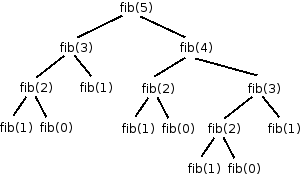
\includegraphics[width=0.5\textwidth]{fib5.png}
\caption{Fibonacci tree}
\end{figure}
We can see that the function fib(3) is being called 2 times. If we would have stored the value of fib(3), then instead of computing it again, we could have reused the old stored value. There are following two different ways to store the values so that these values can be reused:
\begin{enumerate}[label=(\alph*)]
\item Memoization (Top Down)
\item Tabulation (Bottom Up)
\end{enumerate}
So, to use DP, subproblems must be dependent/overlapping. Otherwise, a divide-and-conquer approach is the choice.

\subsection {Tabulation vs Memoization}
\begin{center} \textbf{**Tabulation – Bottom Up Dynamic Programming**} \end{center}
As the name itself suggests starting from the bottom and cumulating answers to the top.Let’s describe a state for our DP problem to be dp[x] with dp[0] as base state and dp[n] as our destination state. So,  we need to find the value of destination state  dp[n].If we start our transition from our base state i.e dp[0] and follow our state transition relation to reach our destination state dp[n], we call it Bottom Up approach as it is quite clear that we started our transition from the bottom base state and reached the top most desired state.
\vspace{3mm}
\begin{lstlisting}
// Bottom up version to find factorial x.
int dp[max];

// base case
int dp[0] = 1;
for (int i = 1; i< =n; i++)
{
    dp[i] = dp[i-1] * i;
}
\end{lstlisting}
The above code clearly follows the bottom-up approach as it starts its transition from the bottom-most base case dp[0] and reaches its destination state dp[n]. Here, we may notice that the dp table is being populated sequentially and we are directly accessing the calculated states from the table itself and hence, we call it tabulation method.
\vspace{3mm}
\begin{center} \textbf{** Memoization Method – Top Down Dynamic Programming**} \end{center}
If we need to find the value for some state say dp[n] and instead of starting from the base state that  dp[0] we ask our answer from the states that can reach the destination state dp[n] following the state transition relation, then it is the top-down fashion of DP. So, we start from dp[n] and to calculate that we go down to dp[n-1] ... ... until we are done calculating and storing dp[0] in this manner. Let's have a look into the code of finding factorial x in this method.
\vspace{3mm}
\begin{lstlisting}
// Top down version to find factorial x.
// To speed up we store the values of calculated states

// initialized to -1
int dp[n]

// return fact x!
int solve(int x)
{
    if (x==0)
        return 1;
    if (dp[x]!=-1)
        return dp[x];
    return (dp[x] = x * solve(x-1));
}
\end{lstlisting}
\vspace{3mm}
As we can see we are storing the most recent solution such a way that if next time we got a call from the same state we simply return it from the memory. So, this is why we call it memoization as we are storing the most recent state values.
\begin{figure}[H]
\centering
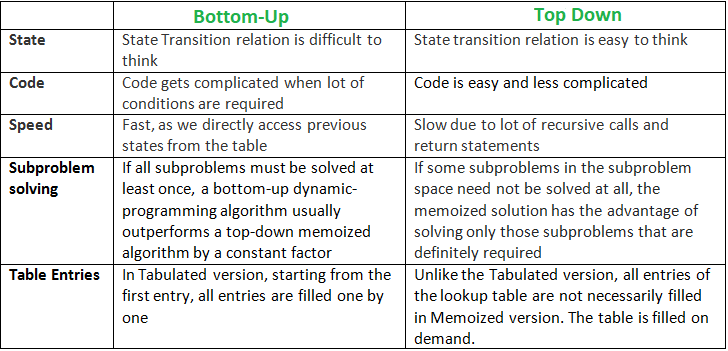
\includegraphics[width=1.0\textwidth]{TabulationvsMemoization.png}
\caption{Comparison between Bottom-up and Top down approach.}
\end{figure}

\section {Examples of Dynamic Programming Problems}
Basic problems -
\begin{enumerate}
\item Fibonacci numbers
\item Tiling Problems
\item Coin change problem
\item Subset sum problem
\item Longest Common Sub-sequence
\item Longest Repeated Subsequence
\item Longest Increasing Subsequence
\item LCS (Longest Common Subsequence) of three strings
\item Warshall’s All pairs shortest path
\item Bellman Ford’s Single Source Shortest Path
\end{enumerate}

Advanced problems - 
\begin{enumerate}
\item Matrix chain multiplication
\item BitMasking
\item Digit DP
\end{enumerate} and so on. Here, we will be discussing about Tiling problem first.

\subsection{Overview on Dynamic programming solving Fibonacci number problem}
The Fibonacci numbers are the numbers in the following integer sequence.\newline
0, 1, 1, 2, 3, 5, 8, 13, 21, 34, 55, 89, 141, ... ... ... \newline
In mathematical terms, the sequence Fn of Fibonacci numbers is defined by the recurrence relation.
\[ F_n =  F_{n-1} + F_{n+2} \]
with seed values
$ F_0 = 0$  and  $ F_1 = 1 $
Write a function int \textbf{fib(int n)} that returns $F_n$ . For example, if n = 0, then fib() should return 0. If n = 1, then it should return 1. For n > 1, it should return $F_{n-1} + F_{n+2} $.
\newline
Following are different methods to get the nth Fibonacci number\vspace{6mm}
\newline
\textbf{Method 1 ( Use recursion )}
\vspace{3mm}
\newline
A simple method that is a direct recusrive implementation mathematical recurance relation given above.
\vspace{3mm}
\begin{lstlisting}
#include<stdio.h>
int fib(int n){
if (n <= 1) return n;
return fib(n-1) + fib(n-2);  // recursive call of fib(n) here 
}
int main (){
int n;

/* Scan n as nth number */
 print(fib(n))  // returns the value from recursive function

return 0;
}
\end{lstlisting}

Time Complexity: T(n) = T(n-1) + T(n-2) which is exponential. \newline
We can observe that this implementation does a lot of repeated work (see the recursion tree from Fig:2 on page 3). So this is a bad implementation for nth Fibonacci number.\newline
Extra Space: O(n) if we consider the fuinction call stack size, otherwise O(1).
\vspace{6mm}
\newline
\textbf{Method 2 ( Use Dynamic Programming )}
\vspace{3mm}
\newline
We can avoid the repeated work done is the method 1 by storing the Fibonacci numbers
calculated so far.
\begin{lstlisting}

int fib(int n){
/* Declare an array to store fibonacci numbers. */
int f[n+1];
int i;


/* 0th and 1st number of the series are 0 and 1*/
f[0] = 0;
f[1] = 1;
for (i = 2; i <= n; i++){
/* Add the previous 2 numbers in the series and store it */
f[i] = f[i-1] + f[i-2];
}
return f[n];
}
int main (){
int n ;
print( fib(n))
return 0;
}
\end{lstlisting}
Time Complexity: O(n)\newline
Extra Space: O(n)
\vspace{6mm}
\newline
\textbf{Method 3 ( Space Otimized Method 2 )}
\vspace{3mm}
\newline
We can optimize the space used in method 2 by storing the previous two numbers only
because that is all we need to get the next Fibannaci number in series.
\vspace{3mm}
\begin{lstlisting}
/* Optimized version function of method 2*/
int fib(int n){
int a = 0, b = 1, c, i;
if( n == 0)
return a;
for (i = 2; i <= n; i++){
c = a + b;
a = b;
b = c;
}
return b;
}

int main (){
int n;
/* scan n*/
/*printf(fib(n))*/
getchar();
return 0;
}
\end{lstlisting}
Time Complexity: O(n)\newline
Extra Space: O(1)
\newline
This problem can also be solved in  O(logN) complexity using optimized Matrix method and 

\section{Tiling Problem}
\vspace{6mm}

In tiling problem, the problem states that,\newline
Given a 2*N board where  N is any integer value, how many ways can you fill it up with given constant size tiles? 
\begin{figure}[H]
\centering
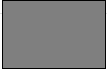
\includegraphics[width=0.24\textwidth]{tile_2xn.png}
\end{figure}
Available tiles 2x1 or 2x2.
\begin{figure}[H]
\centering
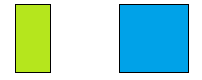
\includegraphics[width=0.25\textwidth]{2x1_2x2.png}
\end{figure}
Now when n = 3 there are 5 possible ways to fill up the board with given tiles. 
\begin{figure}[H]
\centering
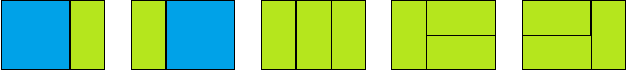
\includegraphics[width=0.5\textwidth]{n3_5.png}
\end{figure}
consider board of width n:
\begin{figure}[H]
\centering
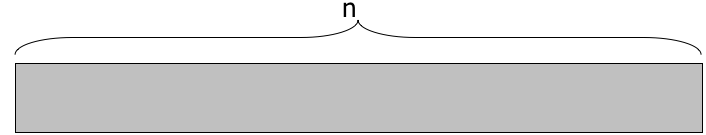
\includegraphics[width=0.5\textwidth]{fn.png}
\end{figure}
So, possible ways to fill the rightmost column :\newline
1. By one 2×1 vertically.
\begin{figure}[H]
\centering
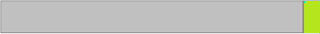
\includegraphics[width=0.5\textwidth]{f1_2x1.png}
\end{figure}
2. By two of 2×1 horizontally.
\begin{figure}[H]
\centering
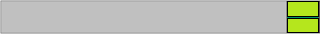
\includegraphics[width=0.5\textwidth]{f2_2x1.png}
\end{figure}
3. By one 2×2 either horizontally or vertically( since both are same).
\begin{figure}[H]
\centering

\includegraphics[width=0.5\textwidth]{f1_2x2.png}
\end{figure}
 Let f(n) be the number of ways of filling a board of size 2×n.
\newline
So,  f(n) = f(n-1) + f(n-2) + f(n-2)
\begin{figure}[H]
\centering

\includegraphics[width=0.5\textwidth]{f1_ways.png}
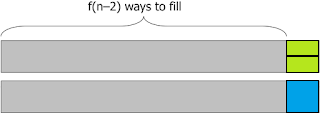
\includegraphics[width=0.5\textwidth]{fn_2ways.png}
\end{figure}
 Now, let's determine the base cases.\newline
\textbf{1.}   f(0) = 1, because if we have to find f(1) then , f(1) = f(0) + f(-1) + f(-1) , since f(-1) not exist, so  f(-1) = 0 then f(1) = f(0) + 0 + 0 => f(1) = f(0) 
since there is one way to fill the board of size 2×1 by using one 2×1 tile. It means that f(0) must 
be equal to 1.
\newline
\textbf{2.}   f(1) = 1
\vspace{6mm}
\newline
\textbf{Algorithm/Code: }
\begin{lstlisting}
int ways[x];

int filling_tiles(int n){
	if(ways[n] != -1) return ways[n];
	return (ways[n] = f(n-1) + 2*f(n-2));
}


int main(){
	ways[0];
	ways[1];
	for(int i =2; i < x ; i++) ways[i] = -1;
//cout << f(x) ;
return f(x)
\end{lstlisting}
\textbf{Complexity:} O(n) \vspace{3mm}
\newline
\textbf{Another problem:} \vspace{3mm}\newline  Suppose this time N = 3 and a tile can be either placed horizontally 1x2 or vertically, 2x1.\newline
For instance,  below is a  board A. How many ways can it be  filled up using tile B(2x1 or 1x2 both are same just rotated)?
\begin{figure}[H]
\centering
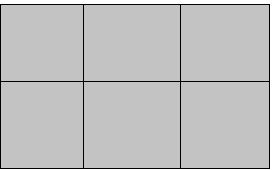
\includegraphics[width=0.3\textwidth]{3.png}
\caption {Board A - 2x3}
\end{figure}
Here N= 3 , so the board in 2x3.
and given tile(s) is 2x1 or 1x2
\begin{figure}[H]
\centering
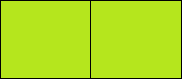
\includegraphics[width=0.20\textwidth]{1x2.png}
\caption{tile B - 1x2}
\end{figure}
\begin{figure}[H]
\centering
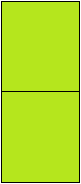
\includegraphics[width=0.10\textwidth]{2x1.png}
\caption{tile B - 2x1}
\end{figure}
2x1 tiles can be placed vertically or horizontally into 2xN tiles. You can place the tiles B on A by the following combinations.
\begin{itemize}
\item All of (2x1) tiles Horizontally
\item (1x2) - Twice vertically and (2x1) -  once horizontally
\item (2x1) -  Twice horizontally and (1x2) - once vertically
\end{itemize}
That’s all the combination possible for three tiles. \vspace{2mm}\newline  
\textbf{What if N was 1?}\newline
The 2x1- board would be as follows: 
\begin{figure}[H]
\centering

\includegraphics[width=0.10\textwidth]{2x1B.png}
\end{figure}
And to overlap all of it, tile-B could be used vertically once only. So, for N = 1 , answer would be one.\newline
\textbf{What if N was 2?}\newline Then the figure(2x2) would be,
\begin{figure}[H]
\centering
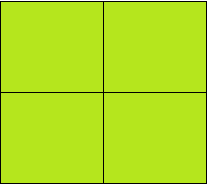
\includegraphics[width=0.25\textwidth]{2x2.png}
\end{figure}
The following possible ways to fill up figure(2x2) using tiles(2x1) are :\newline
--Twice Horizontally\newline
--Twice Vertically\newline
Apart from these two combination, there aren’t any other options. So, for N’s value 2, 2 combinations are possible. 
Because, so far we are getting linear values, the case still remains ambiguous on whether we would always get linear value answers.\newline Now, let’s see the combinations for N’s value 4.
\begin{itemize}
\item All tiles piled horizontally
\item All tiles piled vertically
\item Two horizontally and two vertically
\item Two vertically and two horizontally.
\item First and last horizontally and middle two vertically
\end{itemize}
Those are all the combinations possible for N’s value 4. Notice for 4, the value is 5. If nicely presented, the data would look like below :
\begin{center}
\begin{tabu} to 0.8\textwidth { | X[2] | X[.8] | X[.8] | X[.8]|X[.8]|}
 \hline
 N&1&2&3&4\\
 \hline
 Number of Ways&1&2&3&5  \\
\hline
\end{tabu}
\end{center}
So, as more tiles added, combinations won’t increase linearly. But it seems for N’s value 3, answer could be achieved by adding previous two data together. And same case follows for N’s value 4. We could achieve 5’s combination using previous two values. 
\newline
For this problem, we have base case 1 and 2 for which we could get combination of 1 and 2 respectively. And a function of N can be formed by following way:
\newline
\begin{center}
N(n) = N(n-1) + N(n-2)
\end{center}
Here n is the integer describe 2*n tiles. And n’s data lies in data of n-1 and n-2.
\newline
Algorithm/Pseudo code is provided below: 
\newline
Variables : \newline
n : n is the integer which describes how far horizontally our input explores. 2*n.\newline
Dp[i] : for any integer number i,\vspace{3mm}\newline Here, Dp[i] stores the value of ith integer combination of way tiling input \vspace{3mm}
\newline
Code: \vspace{3mm}
\begin{lstlisting}
Filling-Tiles (n)
{
    if(n is 1)
return 1; //base case one
    If (n is 2)
   	 return 2; // base case 2
   if (n is 3)
	return 3; //base case 3
else {

  	  Filling-Tiles (n) = Filling-Tiles (n-1) +   Filling-Tiles (n-2);
  	  //This recursively calls for the value of n-1 and n-2 and sends the summation as answer;
         }
}
\end{lstlisting}
Time Complexity: O(n)
\newline
Memory Complexity: O(n)
\newline
\vspace{6mm}
\section{Flag/Coloring Problem}
Coloring flag is a common dynamic programming problem for beginners.
It can be solved using basic math too  but for beginners DP (short for dynamic programming) learners, it’s better to avoid math in this case.\vspace{2mm}
\newline
The problem statement is as follows below:\vspace{3mm} \newline
Given three colors, white, red and blue, how many way can you fill up a  sequence, provided the length of the sequence? Also, you can’t have any 2 same colors in adjacent cells. As in, the tiles may not be Red and Red, or White and White. It has to be Red and White or White and Red. Also to make the task more difficult, you may put \textbf{Blue} only between\textbf{ Red} and \textbf{White} or White and Red. The length of the sequence of to be colored will be provided in integer number n.\vspace{3mm}
\newline
For instance, if N is 1, then how many ways can you fill up the one cell? 
\begin{figure}[H]
\centering
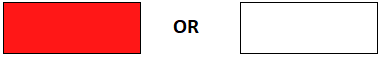
\includegraphics[width=0.50\textwidth]{row.png}
\end{figure}
Possible answer is red or white. So for N equals to 1, the answer is 2.\vspace{9mm}\newline
\textbf{What if N is 2?}\vspace{3mm}\newline 
We can either choose Red and White combination or choose White and Red combination.
\begin{figure}[H]
\minipage{0.45\textwidth}

\includegraphics[width=\linewidth]{rw.png}
\caption{Red and White combination}
\endminipage\hfill
\minipage{0.45\textwidth}%

\includegraphics[width=\linewidth]{wr.png}
\caption{White and Red combination}
\endminipage
\end{figure}
The primary step of solving a problem using  DP is understanding what the problem is about and what it’s asking. Then figuring out what could be the base cases, or constant cases. And these cases could be set as default cases. These cases could be used to solve for any test case may be given. For this particular problem,  for N = 1, answer will be 2 and for N = 2 answer will be 2. The two best cases which could potentially help further figure out a solution.\vspace{8mm} 
\newline
Now,\textbf{ what would be the result if N was 3?}\vspace{3mm}\newline
For sequence of 3 cells, blue must be used between Red and White or White and Red color. So, that’s already two of the possible combinations we could have. But getting a combination of Red and White or White and Red is acceptable too where two flags/blocks of the same color are not adjacent. So, Red-Red-white or white-white-red is not acceptable. \vspace{3mm}
\newline
So, below are the possible combinations we should come up with for N’s value 3.
\begin{figure}[H]
\centering

\includegraphics[width=0.40\textwidth]{rbw.png}
\vspace{3mm}

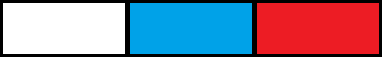
\includegraphics[width=0.40\textwidth]{wbr.png}
\vspace{3mm}


\includegraphics[width=0.40\textwidth]{rwr.png}
\vspace{3mm}

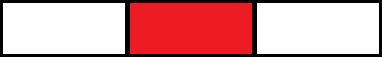
\includegraphics[width=0.40\textwidth]{wrw.png}
\end{figure}
We figuared the combinations out above manually. Now, to demonstrate why base cases are important, let’s further explore what combinations we could form for N’s value 4.\vspace{3mm}\newline
 The possible combination for a sequence of four cells should be like following:
\begin{figure}[H]
\centering
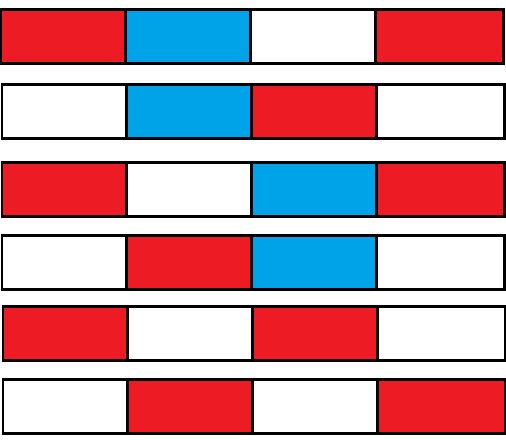
\includegraphics[width=0.50\textwidth]{n4wrb.png}
\caption{All possible combination for N = 4}
\end{figure}
Now, if we check the table of the results for different values of n, we see -
\begin{center}
\begin{tabu} to 1.0\textwidth { | X[2.8] | X[.8] | X[.8] | X[.8]|X[.8]|}
 \hline
 N&1&2&3&4\\
 \hline
 Possible no. of combinations&1&2&4&6 \\
\hline
\end{tabu}
\end{center}
\vspace{6mm}
Dynamic programming is very important to programmers because it saves time and memory. Data can be stored to use later. Previously stored data can be used to find new data. For instance, for the two bases above, 1 and 2, answers are 2 and 2 respectively.  For N’s value 3, answer is 4. Which, as manually demonstrated, was 4 but it  can  also be achieved by adding previous two answers. The answer found for 4 manually was 6. You could add previous two values, 4 and 2 to get the value for 4.\vspace{8mm}\newline
So, it can be deducted that, for this particular problem we can have the formula below:
\[N (4) = N(3) + N(2)\]
\[N (3) = N(3) + N(2)\]
\[...\]
\[...\]
Let’s call this a function of N. For $n^{th}$ value of N,  solve for function N(n) where 
\[N(n) = N (n-1)+ N(n-2)\] 
\newline
Dynamic programming is a very important part of Algorithm 1 course. And most programmers prefer this method if given the choice.  You can solve these type of problems using recursion or loop. But it is better to use recursion. \vspace{3mm}
\newline
Pseudo code is provided below:\vspace{8mm} \newline
Variables :\newline
n : nth sequence for which, find number of combinations\newline
dp[i] : for any integer number i, dp[i] stores the combination which could be used to color i cells.\newline
 
\textbf{Code:}
\begin{lstlisting}
Flag-Color(n)
{
    if(n is 1 or n is 2)
    return 2;
      // this is the base case
Else {

  	  Flag-Color (n) = Flag-Color(n-1) +   Flag-Color(n-2);
  	  //This recursively calls for the value of n-1 and n-2 and sends the summation as answer;
         }
}
\end{lstlisting}

Time Complexity: O(n)
\newline
Memory Complexity: O(n)
\vspace{16mm}
\newline
\textbf{Resources:}
\newline
\begin{itemize}
\item  http://web.mit.edu/15.053/www/AMP-Chapter-11.pdf
\item  https://web.stanford.edu/class/cs97si/04-dynamic-programming.pdf
\item  https://www.rand.org/content/dam/rand/pubs/papers/2008/P550.pdf
\item  https://www.geeksforgeeks.org/dynamic-programming/
\item  CLRS book 3rd edition
\item  https://www.quora.com/What-are-some-beginner-level-dynamic-programming-problems-that-one-can-try-practicing-on-CodeChef-and-other-online-judges
\end{itemize}
\vspace{10mm}
- - - - - - - - - - - - - - - - - - - - - - - - - - - - - - * - - - - - - - - - - - - - - - - - - - - - - - - - - - - - - - - 
\end{document}